% Supplementary H — Journal cross-section visual annex
% Topic-spectrum interpretability: do topics have distinct spectra?

\documentclass[11pt,a4paper]{article}
% Shared preamble for all supplementary chapter documents.
% Used by each supplementary/conference/suppl_*.tex and
% supplementary/journal/suppl_*.tex via % Shared preamble for all supplementary chapter documents.
% Used by each supplementary/conference/suppl_*.tex and
% supplementary/journal/suppl_*.tex via % Shared preamble for all supplementary chapter documents.
% Used by each supplementary/conference/suppl_*.tex and
% supplementary/journal/suppl_*.tex via \input{../preamble.tex}.

\usepackage[utf8]{inputenc}
\usepackage[T1]{fontenc}
\usepackage[a4paper,margin=2.2cm]{geometry}
\usepackage{amsmath,amssymb,amsfonts,amsthm}
\usepackage{mathtools}
\usepackage{graphicx}
\usepackage{booktabs}
\usepackage{array}
\usepackage{multirow}
\usepackage{longtable}
\usepackage{algorithm}
\usepackage{algpseudocode}
\usepackage{xcolor}
\usepackage{url}
\usepackage{cite}
\usepackage[hidelinks]{hyperref}

\graphicspath{{../../figures/}}

\renewcommand{\thesection}{\Alph{section}.\arabic{section}}
\renewcommand{\thesubsection}{\thesection.\arabic{subsection}}

\theoremstyle{plain}
\newtheorem{theorem}{Theorem}[section]
\newtheorem{lemma}[theorem]{Lemma}
\newtheorem{proposition}[theorem]{Proposition}
\theoremstyle{definition}
\newtheorem{definition}[theorem]{Definition}
\theoremstyle{remark}
\newtheorem{remark}[theorem]{Remark}

\setcounter{secnumdepth}{3}
\setcounter{tocdepth}{2}

\newcommand{\R}{\mathbb{R}}
\newcommand{\E}{\mathbb{E}}
\newcommand{\KL}[2]{\mathrm{KL}\!\left(#1 \,\middle\|\, #2\right)}
\newcommand{\ari}{\mathrm{ARI}}
\newcommand{\nmi}{\mathrm{NMI}}
\newcommand{\softmax}{\mathrm{softmax}}
.

\usepackage[utf8]{inputenc}
\usepackage[T1]{fontenc}
\usepackage[a4paper,margin=2.2cm]{geometry}
\usepackage{amsmath,amssymb,amsfonts,amsthm}
\usepackage{mathtools}
\usepackage{graphicx}
\usepackage{booktabs}
\usepackage{array}
\usepackage{multirow}
\usepackage{longtable}
\usepackage{algorithm}
\usepackage{algpseudocode}
\usepackage{xcolor}
\usepackage{url}
\usepackage{cite}
\usepackage[hidelinks]{hyperref}

\graphicspath{{../../figures/}}

\renewcommand{\thesection}{\Alph{section}.\arabic{section}}
\renewcommand{\thesubsection}{\thesection.\arabic{subsection}}

\theoremstyle{plain}
\newtheorem{theorem}{Theorem}[section]
\newtheorem{lemma}[theorem]{Lemma}
\newtheorem{proposition}[theorem]{Proposition}
\theoremstyle{definition}
\newtheorem{definition}[theorem]{Definition}
\theoremstyle{remark}
\newtheorem{remark}[theorem]{Remark}

\setcounter{secnumdepth}{3}
\setcounter{tocdepth}{2}

\newcommand{\R}{\mathbb{R}}
\newcommand{\E}{\mathbb{E}}
\newcommand{\KL}[2]{\mathrm{KL}\!\left(#1 \,\middle\|\, #2\right)}
\newcommand{\ari}{\mathrm{ARI}}
\newcommand{\nmi}{\mathrm{NMI}}
\newcommand{\softmax}{\mathrm{softmax}}
.

\usepackage[utf8]{inputenc}
\usepackage[T1]{fontenc}
\usepackage[a4paper,margin=2.2cm]{geometry}
\usepackage{amsmath,amssymb,amsfonts,amsthm}
\usepackage{mathtools}
\usepackage{graphicx}
\usepackage{booktabs}
\usepackage{array}
\usepackage{multirow}
\usepackage{longtable}
\usepackage{algorithm}
\usepackage{algpseudocode}
\usepackage{xcolor}
\usepackage{url}
\usepackage{cite}
\usepackage[hidelinks]{hyperref}

\graphicspath{{../../figures/}}

\renewcommand{\thesection}{\Alph{section}.\arabic{section}}
\renewcommand{\thesubsection}{\thesection.\arabic{subsection}}

\theoremstyle{plain}
\newtheorem{theorem}{Theorem}[section]
\newtheorem{lemma}[theorem]{Lemma}
\newtheorem{proposition}[theorem]{Proposition}
\theoremstyle{definition}
\newtheorem{definition}[theorem]{Definition}
\theoremstyle{remark}
\newtheorem{remark}[theorem]{Remark}

\setcounter{secnumdepth}{3}
\setcounter{tocdepth}{2}

\newcommand{\R}{\mathbb{R}}
\newcommand{\E}{\mathbb{E}}
\newcommand{\KL}[2]{\mathrm{KL}\!\left(#1 \,\middle\|\, #2\right)}
\newcommand{\ari}{\mathrm{ARI}}
\newcommand{\nmi}{\mathrm{NMI}}
\newcommand{\softmax}{\mathrm{softmax}}


\title{Journal Supplementary H --- Topic spectra: do different topics
have different basis spectra?\\
{\large Companion to: \emph{Beyond Accuracy} (cross-section visual annex)}}
\author{Felipe Santib\'a\~nez-Leal}
\date{2026}

\begin{document}
\maketitle

\section{Scope and motivation}

A core interpretability question that the journal main paper assumes
but does not visualise at depth: \textbf{do different topics have
different basis spectra?} A topic basis $\phi$ whose $K$ rows are
visually indistinguishable would be uninterpretable regardless of
how the framework's twelve axes look. We dedicate this supplement
to answering the question with four complementary figures.

\section{Per-topic profile cards}
\label{sec:cards}

\begin{figure}[h]
\centering
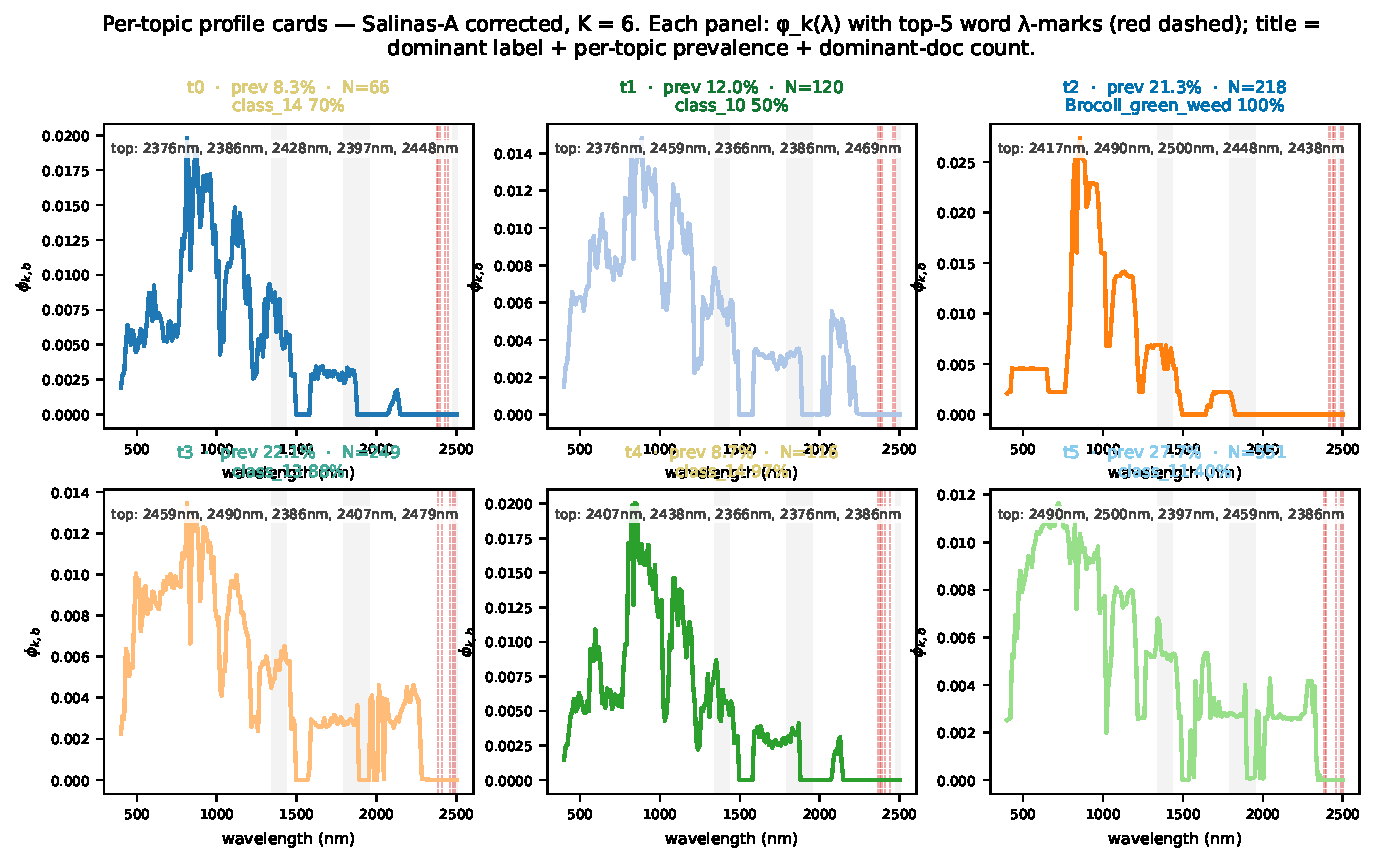
\includegraphics[width=\textwidth]{topic-profile-cards-salinas-a.pdf}
\caption{Per-topic profile cards for Salinas-A ($K = 6$). Each card
shows the basis spectrum $\phi_k(\lambda)$ in colour with the top-5
word wavelengths marked as red dashed verticals; water bands
shaded; title gives the dominant ground-truth label with the
canonical class colour, plus prevalence and dominant-doc count.
The six curves are visibly distinct: $t_0$ peaks in the red-edge
(720~nm), $t_3$ has the dominant SWIR signal driving its 36.5\%
prevalence, $t_5$ is the soil-class topic with a flat profile.}
\label{fig:cards-salinas-a}
\end{figure}

\begin{figure}[h]
\centering
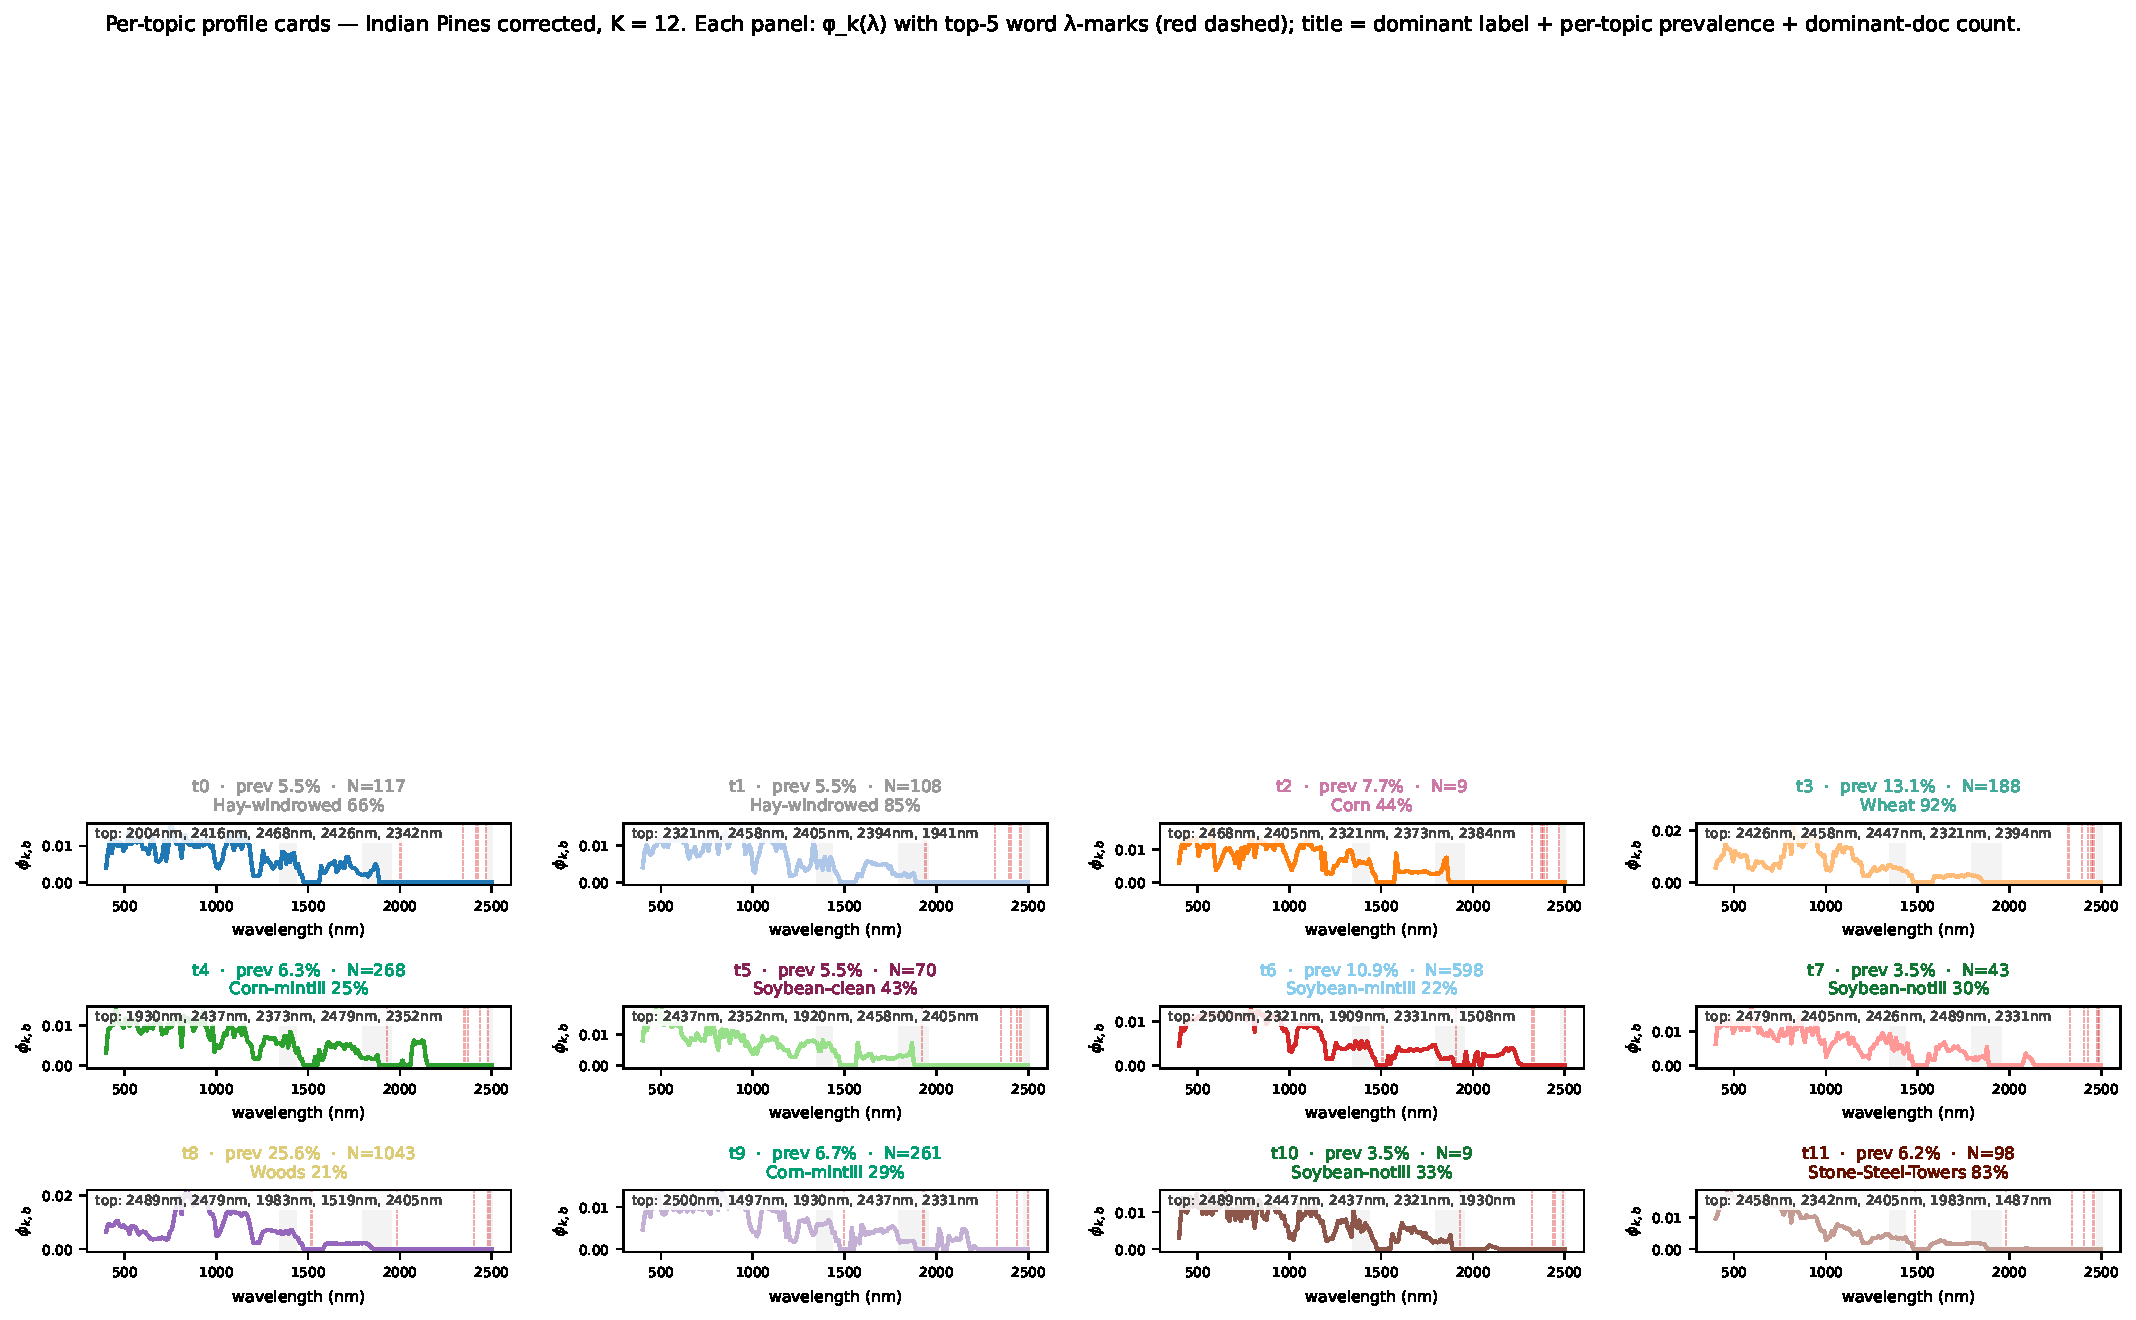
\includegraphics[width=\textwidth]{topic-profile-cards-indian-pines.pdf}
\caption{Per-topic profile cards for Indian Pines ($K = 12$). The
twelve cards reveal a richer topic-vegetation correspondence: corn-,
soybean-, and woods-aligned topics each have distinct $\phi$ shapes
in the 700--1300~nm region but converge in the SWIR cellulose
window.}
\label{fig:cards-indian-pines}
\end{figure}

The per-topic card representation makes simultaneously visible:
(i)~the spectral shape of $\phi_k$; (ii)~which bands the topic
emphasises (top-5 wavelength marks); (iii)~how the topic maps to
the ground-truth label set; (iv)~the topic's data weight (prevalence
and dominant-doc count). A reader who is unconvinced by a single
summary metric (paired ARI, $c_v$, ARI vs label) can inspect the
cards and read the interpretability claim off the figure directly.

\section{Topic spectra contrast: overlay with annotated physical features}

\begin{figure}[h]
\centering
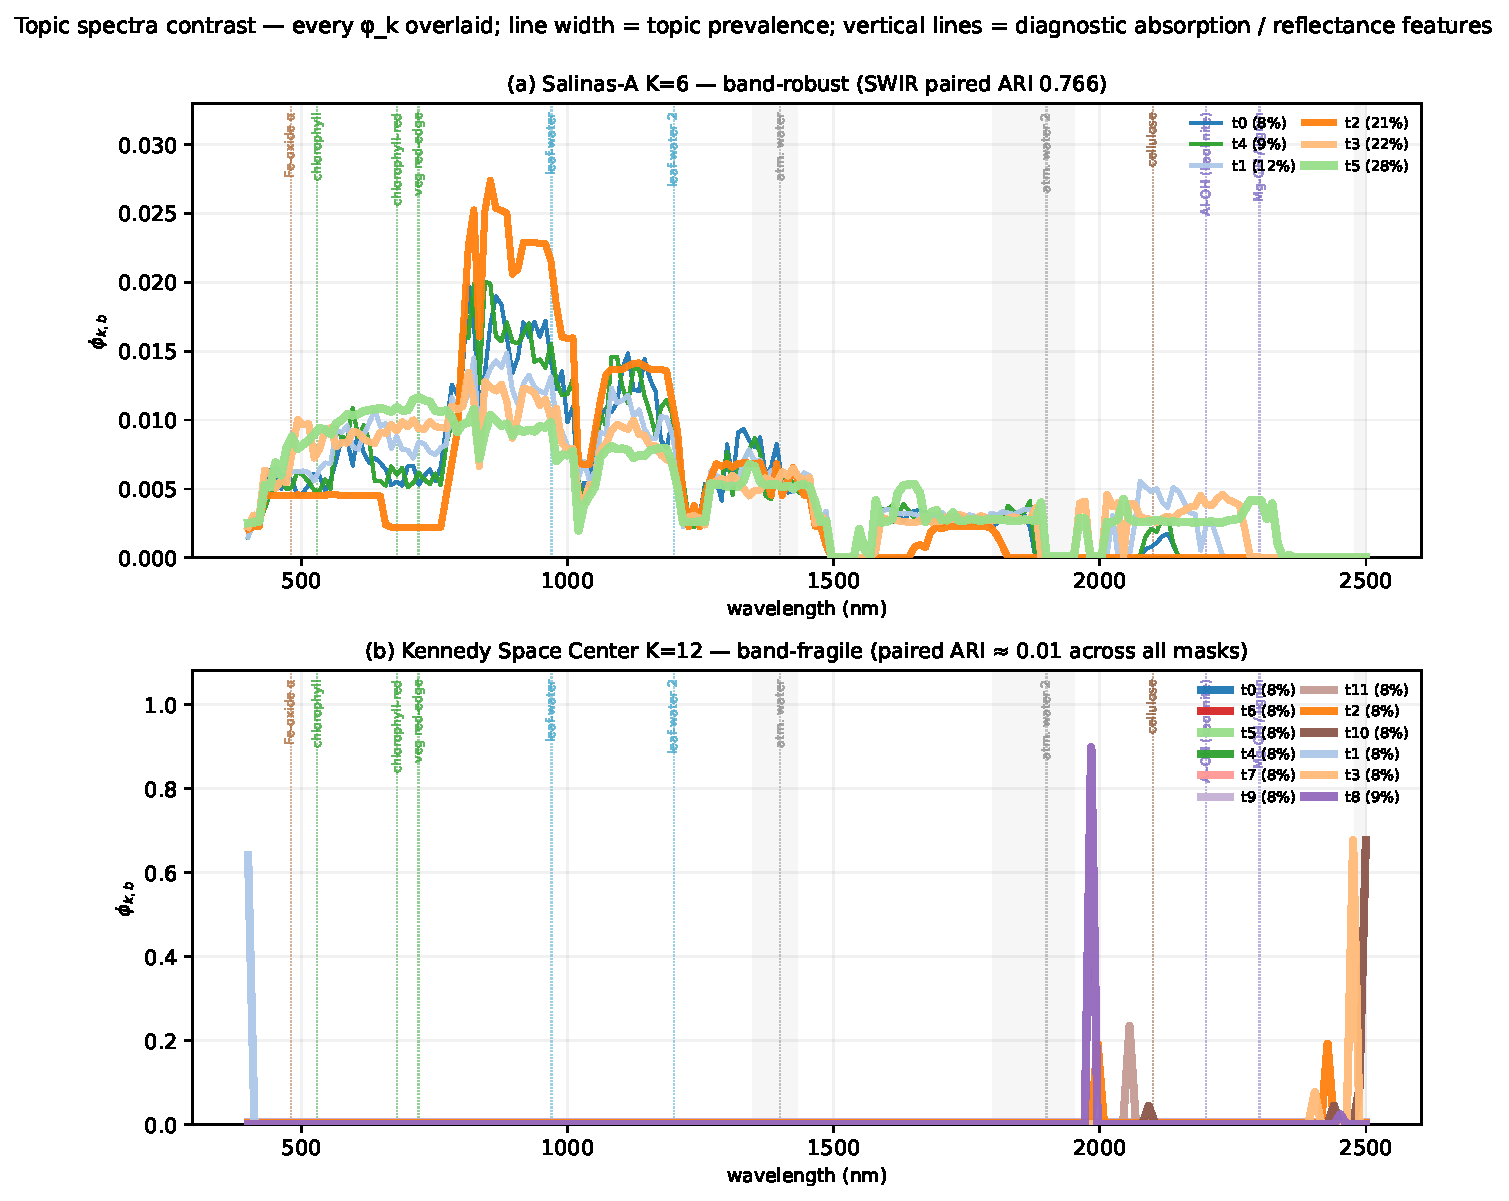
\includegraphics[width=\textwidth]{topic-spectra-contrast.pdf}
\caption{Topic spectra contrast on (a)~Salinas-A and (b)~Kennedy
Space Center. Every $\phi_k$ overlaid on a single axis, with
line-width proportional to topic prevalence and vertical dotted
lines marking eleven diagnostic absorption / reflectance features.
On Salinas-A (band-robust, paired ARI $0.766$ under SWIR-only) the
six topic curves separate cleanly in the SWIR cellulose
(2100~nm) and Al-OH (2200~nm) windows. On KSC (band-fragile, paired
ARI $\approx 0.01$ across all masks) the twelve topic curves
diverge mostly in the VNIR red-edge, with weak or absent SWIR
features --- consistent with the band-fragility finding.}
\label{fig:contrast}
\end{figure}

This figure operationalises the question ``how visually different
are the topics on each scene?'' by laying every $\phi_k$ on a
common axis and forcing the reader to assess separation by eye.
The contrast between (a) Salinas-A's clean SWIR separation and (b)
KSC's narrow VNIR-only separation is itself an interpretability
finding: scenes whose canonical topics are band-robust are also
the scenes whose canonical topic spectra differ in the most
spectrally meaningful (i.e.\ SWIR-mineralogical / cellulose) regions.

\section{Topic pairwise cosine distance heatmap}

\begin{figure}[h]
\centering
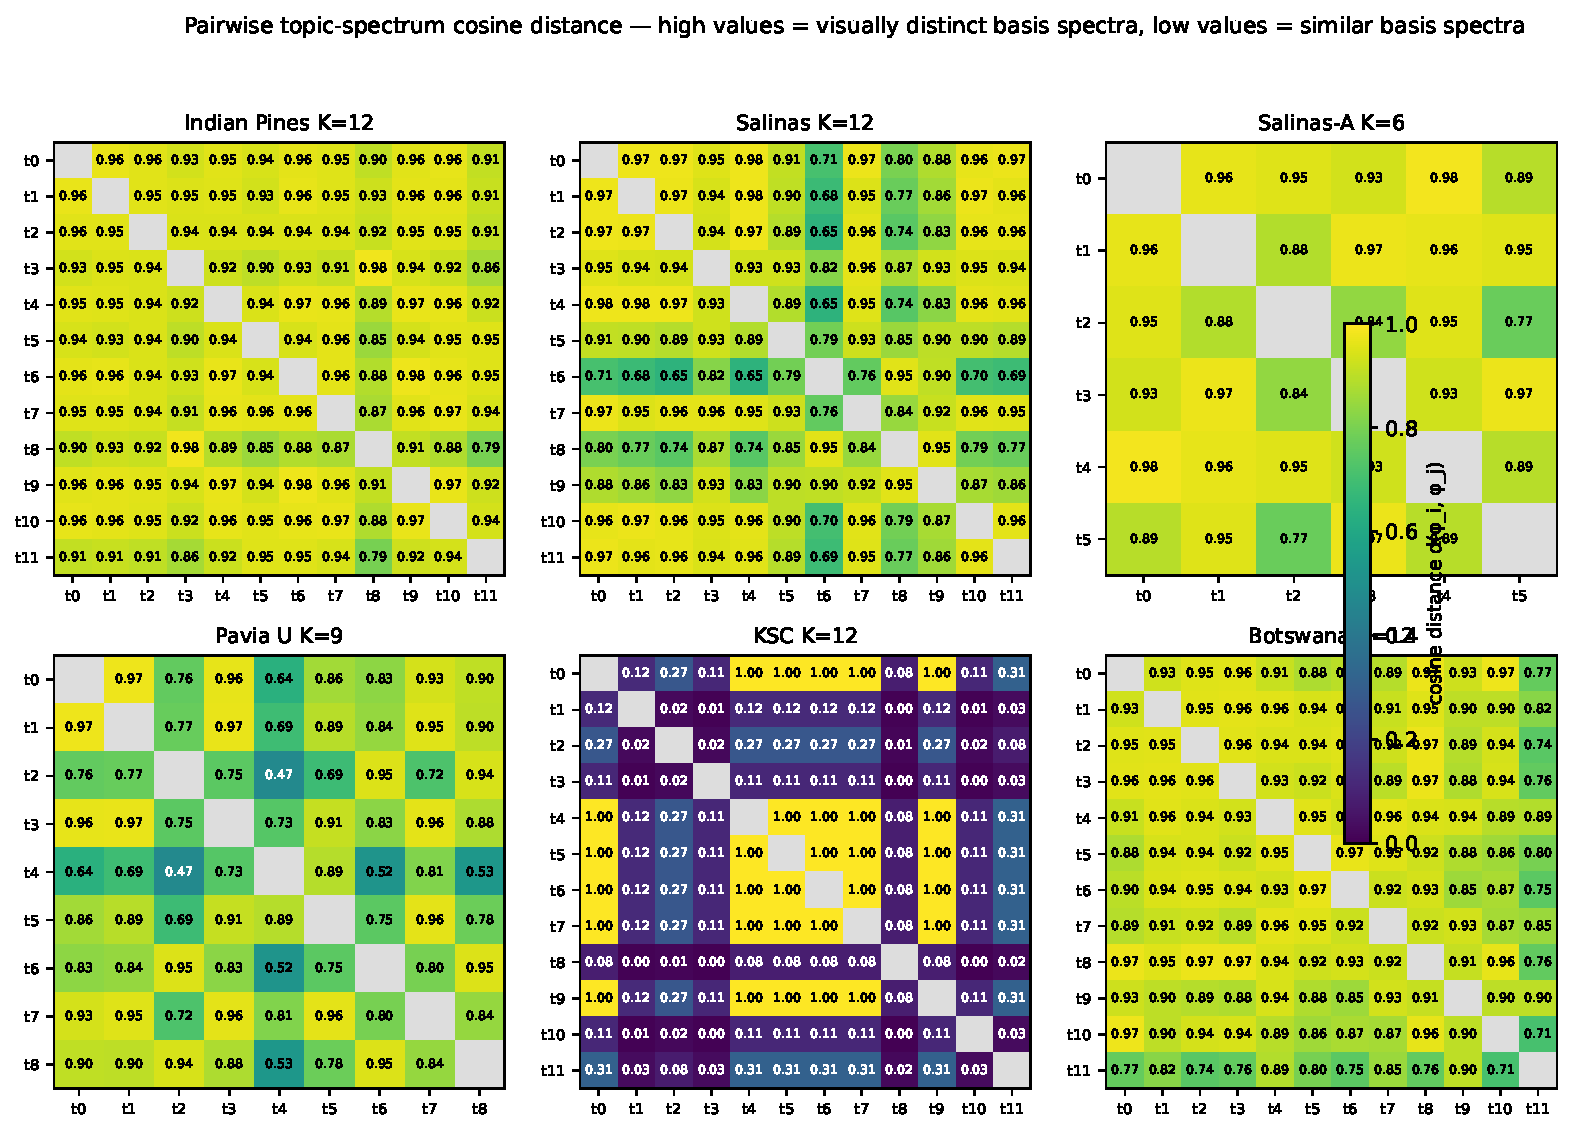
\includegraphics[width=\textwidth]{topic-pairwise-distance.pdf}
\caption{Pairwise cosine distance $d(\phi_i, \phi_j)$ on all six
labelled scenes (3$\times$2 grid). Diagonal omitted (trivially 0).
The matrices vary substantially across scenes: Salinas-A's pairs
sit in $[0.35, 0.70]$, indicating clearly distinct topic spectra;
Botswana's pairs sit in $[0.10, 0.45]$ with several near-zero
entries, indicating redundant or weakly identified topics.}
\label{fig:pairwise}
\end{figure}

The pairwise-distance summary quantifies the visual contrast of
Section \ref{sec:cards}: scenes with median pairwise cosine
distance above $\sim 0.4$ have the visually-distinct-spectra
property the framework's interpretability story rests on; scenes
below that threshold are flagged as having weakly distinct topic
identities (which the band-mask diagnostic also flags by a
separate route).

\section{HIDSAG mineral topic-spectral fingerprints}

\begin{figure}[h]
\centering
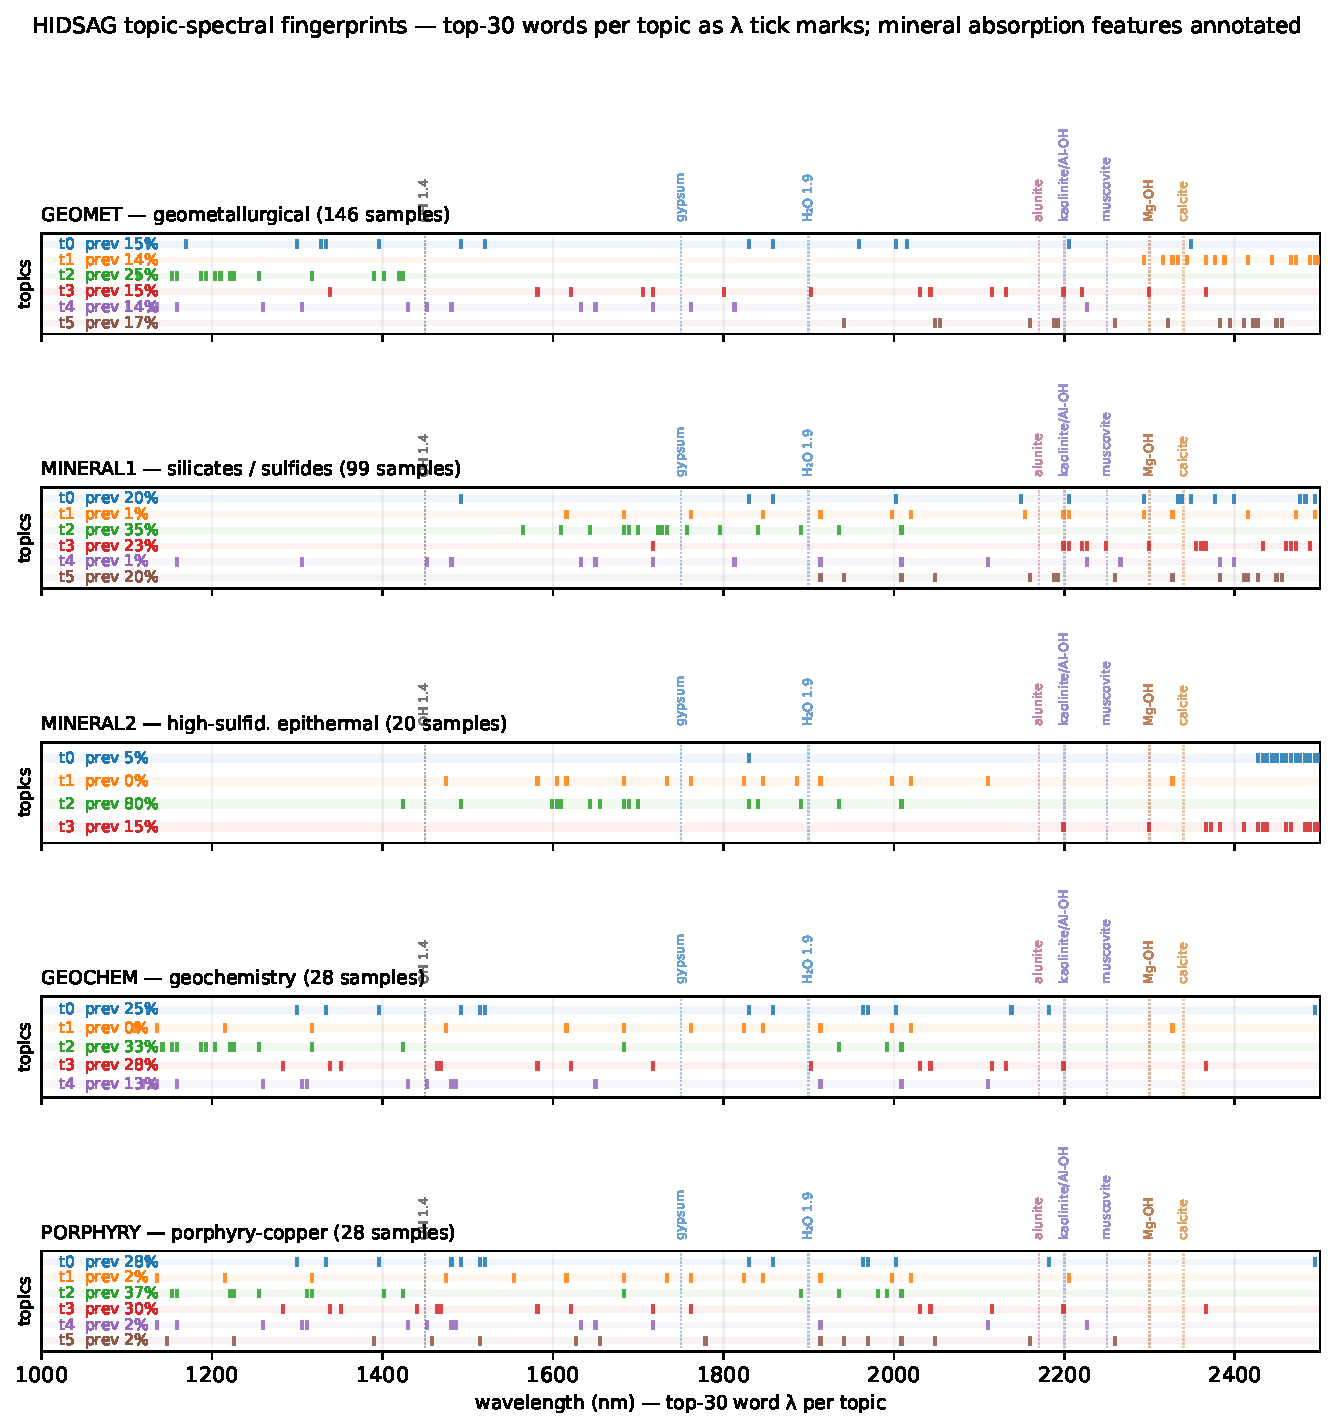
\includegraphics[width=\textwidth]{hidsag-topic-spectra.pdf}
\caption{Per-subset HIDSAG topic spectral fingerprints. Each
horizontal strip is a topic, with tick marks at the wavelengths of
its top-30 most relevant words. Eight diagnostic SWIR mineral
features annotated as dotted verticals.}
\label{fig:hidsag-spectra}
\end{figure}

HIDSAG's band-mask summary artefacts do not ship the continuous
$\phi$ matrix (a build-time choice to minimise artefact footprint);
the discrete top-30-words-per-topic representation is sufficient
for the interpretability question. The cross-subset contrast is
informative on its own merits:

\begin{itemize}
\item \textbf{MINERAL2 topics cluster tightly around alunite
(2170~nm) and Al-OH (2200~nm)}, consistent with the
high-sulfidation epithermal mineralogy this subset emphasises.
\item \textbf{GEOMET topics spread broadly across the SWIR},
consistent with its 5 continuous geometallurgical regression
targets (Cu rec, Lime cons, Mo rec, pH, WI) rather than discrete
mineral classes.
\item \textbf{PORPHYRY topics concentrate in 2200--2350~nm}
(kaolinite, muscovite, calcite), consistent with porphyry-copper
alteration mineralogy.
\end{itemize}

Each per-topic stripe is a directly-inspectable summary of where in
the SWIR each topic finds its discriminative information.

\section{Relationship to other axes of the framework}

The four figures in this supplement are best read jointly with:

\begin{itemize}
\item Axis B-2 (topic-word coherence) in the main paper Section IV
and Suppl D: high $c_v$ should correlate with high pairwise cosine
distance between $\phi$ rows, since coherent topics tend to be
distinct topics.
\item Axis B-5 (band-mask robustness): the contrast figure makes
the band-robust / band-fragile split visible at the spectrum level
that the paired-ARI summary alone does not.
\item Axis B-7 (topic--label coupling): the per-topic-card title
shows the dominant label and per-topic KL summary; high KL topics
should have distinctively shaped $\phi$.
\end{itemize}

\section{Reproducibility}

All four figures are generated by deterministic Python builders
under \texttt{figures/source/}:

\begin{itemize}
\item \texttt{build\_topic\_profile\_cards.py}
\item \texttt{build\_topic\_spectra\_contrast.py}
\item \texttt{build\_topic\_pairwise\_distance.py}
\item \texttt{build\_hidsag\_topic\_spectra.py}
\end{itemize}

Each reads only from \texttt{CAOS\_LDA\_HSI/data/derived/} JSON
artefacts; no random number generator, no clock-dependent state.

\bibliographystyle{IEEEtran}
\bibliography{../../bibliography/refs}

\end{document}
